%!TEX root = ../main.tex

\chapter{Einleitung} % (fold)
\label{chapter:einleitung}

Als Polymer bezeichnet man einen aus Makromolekülen bestehenden Stoff.
Diese Makromoleküle setzen sich wiederum aus vielen kleineren sich wiederholenden Molekülen, in diesem Zusammenhang Monomere genannt, zusammen.
Besteht ein Polymer aus nur einer Monomer-Gattung, dann spricht man von einem Homopolymer, sonst von einem Heteropolymer oder auch Copolymer.
Obwohl Polymere in vielen verschiedenen Konfigurationen, beispielsweise ring- oder sternförmig, auftreten können, beschränken wir uns hier auf den Fall eines kettenförmigen Aufbaus.
Weiter interessieren wir uns hier nur für Copolymere, vor allem die sogenannten Blockcopolymere, welche aus mehreren Monomer-Gattungen, die homogene zusammenhängende Blöcke bilden, aufgebaut sind; siehe \cref{figure:polymerketten}.

\begin{figure}[tb]
    \centering
    \begin{subfigure}[b]{\textwidth}
        \centering
        \includestandalone[width=0.7\textwidth]{tikz/einleitung/fig1}
    \end{subfigure}
    \\[0.33em]
    \begin{subfigure}[b]{\textwidth}
        \centering
        \includestandalone[width=0.7\textwidth]{tikz/einleitung/fig2}
    \end{subfigure}
    \\[0.33em]
    \begin{subfigure}[b]{\textwidth}
        \centering
        \includestandalone[width=0.7\textwidth]{tikz/einleitung/fig3}
    \end{subfigure}
    \caption[Skizzenhafte Darstellung verschiedener Polymerarten]{%
        Skizzenhafte Darstellung verschiedener Polymerarten.
        Von oben nach unten: Homopolymer, ein AB-Diblockcopolymer und ein sogenanntes statistisches AB-Copolymer, bei dem die beiden Monomer-Arten zufällig verteilt sind.
    }
    \label{figure:polymerketten}
\end{figure}

Von besonderem Interesse ist nun das Verhalten von Polymerschmelzen (\foreign{engl.}{polymer melt}), das heißt, des flüssigen Aggregatzustands eines Polymers, sowie das Verhalten von Gemischen verschiedener polymerer Stoffe.
So neigen die Gemische vieler Paare von Homopolymeren zu makroskopischer Phasenseparation, wie man es beispielsweise auch von Öl und Essig kennt.
Eine ähnliche Tendenz zur Separation findet man auch bei Schmelzen von Blockcopolymeren, hierbei ist aber aufgrund der Verbindung zwischen den verschiedenen Monomer-Blöcken keine makroskopische Phasenseparation möglich, stattdessen kommt es zu einer periodischen mikroskopischen Separation, vergleiche \cref{figure:phasen}.

Da die experimentelle Bestimmung ohne Vorwissen über mögliche stabile Anordnungen nur wenig erfolgversprechend ist, wird ein theoretisches Fundament benötigt, auf Basis dessen Vorhersagen getroffen werden können, die vorzugsweise auch zu experimentell belegbaren Anordnungen führen.
Wir beschränken uns auf die Betrachtung von Diblockcopolymeren, das heißt, Blockcopolymeren, die aus zwei verschiedenen Monomer-Gattungen bestehen, da diese ein vergleichsweise einfaches System darstellen.

Als nützliches und relativ gut handhabbares theoretisches Modell hat sich die sogenannte \ac{scft} herausgestellt, auf welche wir nun zuarbeiten.

\begin{figure}[tb]
    \centering
    \begin{subfigure}[b]{0.15\textwidth}
        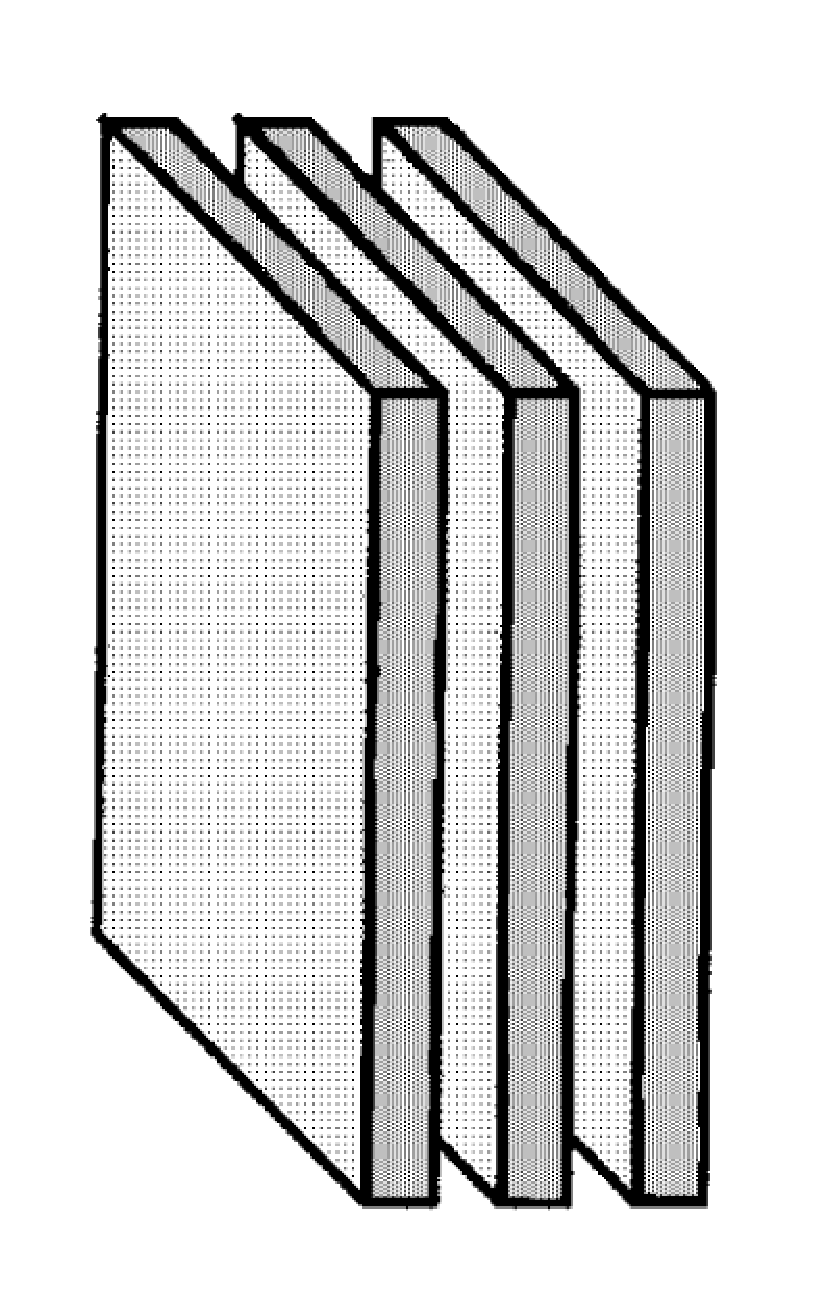
\includegraphics[width=\textwidth]{figures/einleitung/fig1}
    \end{subfigure}
    \begin{subfigure}[b]{0.15\textwidth}
        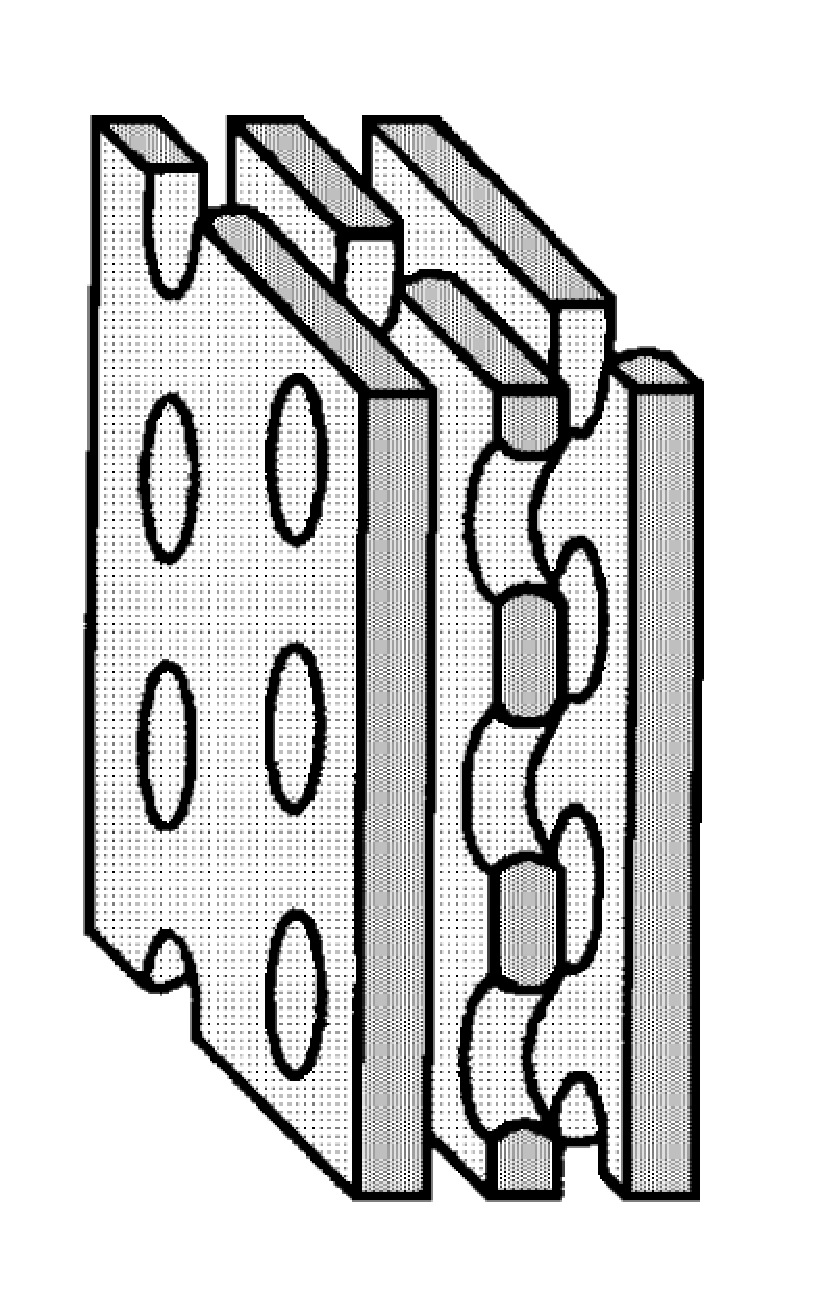
\includegraphics[width=\textwidth]{figures/einleitung/fig2}
    \end{subfigure}
    \begin{subfigure}[b]{0.15\textwidth}
        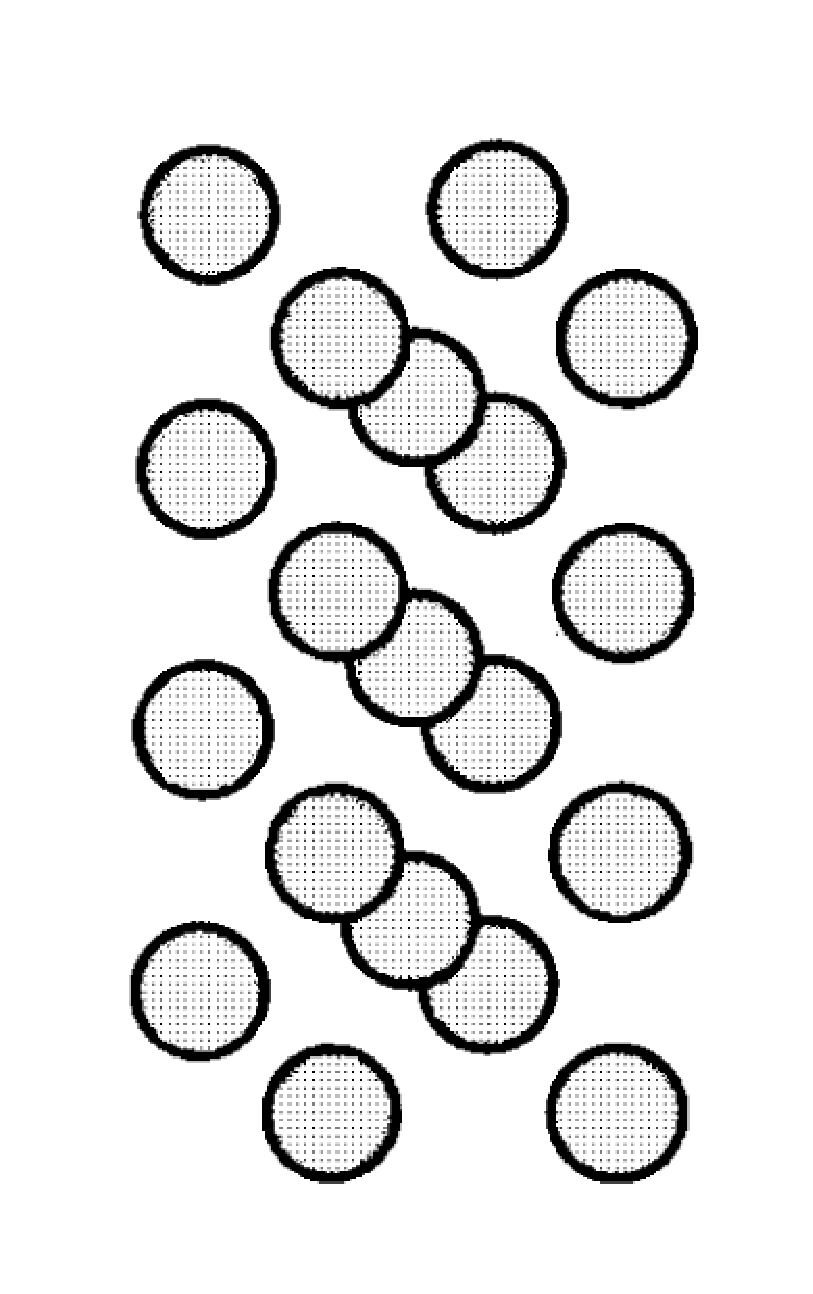
\includegraphics[width=\textwidth]{figures/einleitung/fig3}
    \end{subfigure}
    \begin{subfigure}[b]{0.15\textwidth}
        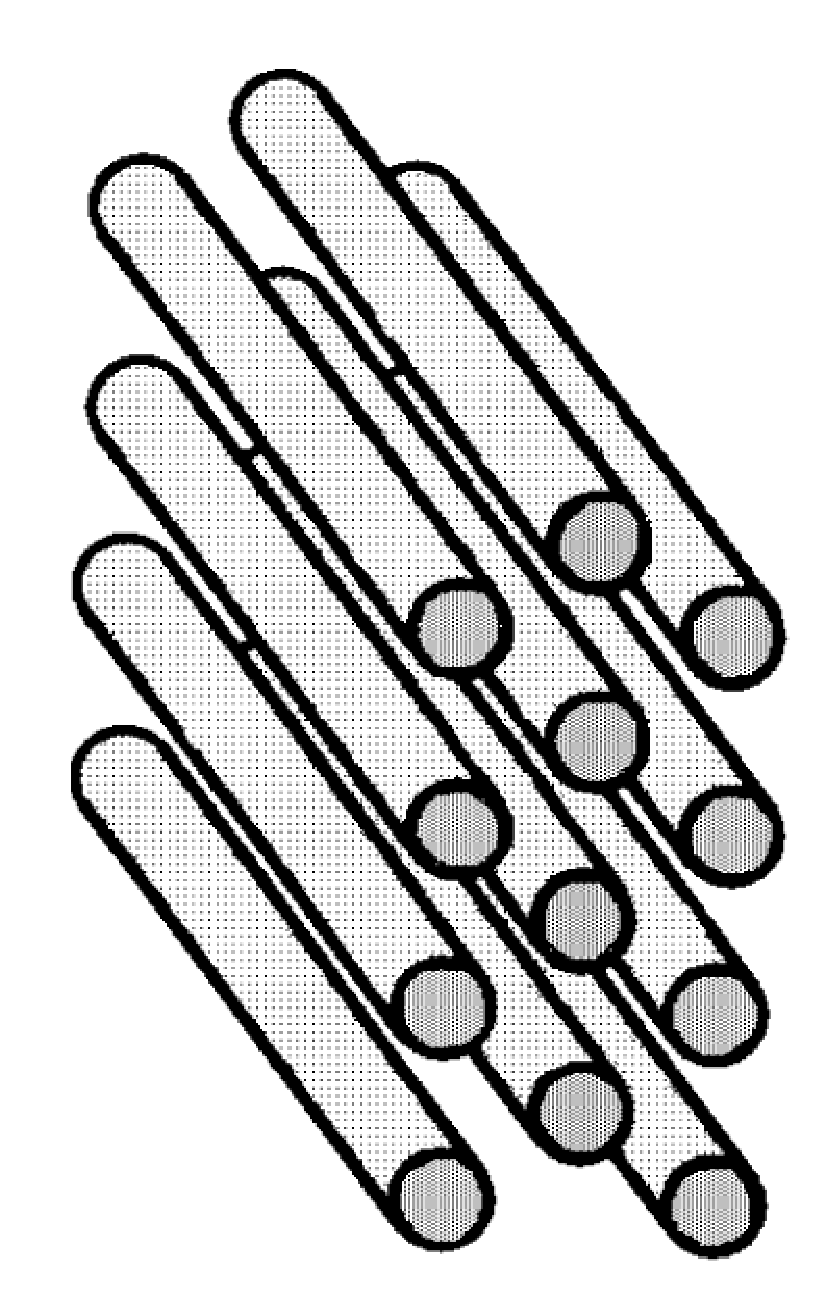
\includegraphics[width=\textwidth]{figures/einleitung/fig4}
    \end{subfigure}
    \begin{subfigure}[b]{0.15\textwidth}
        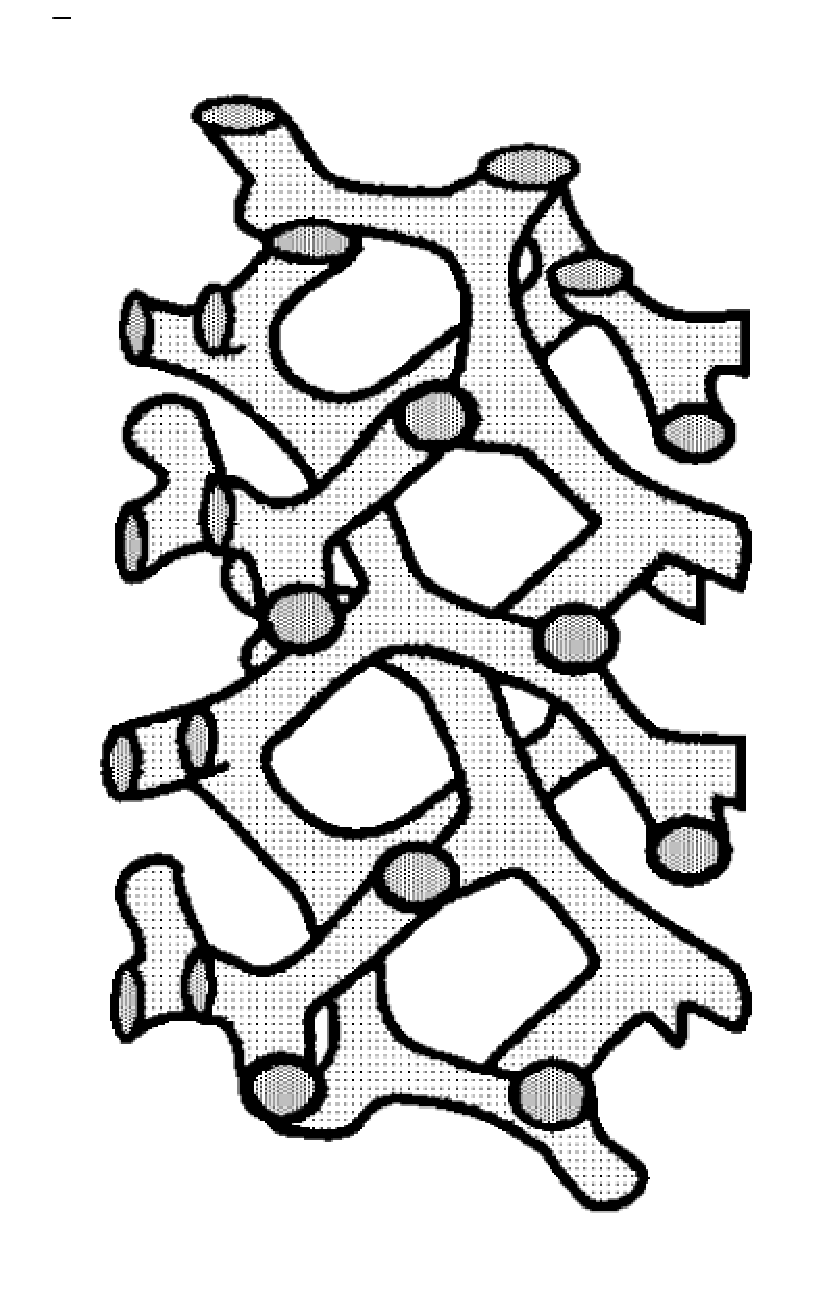
\includegraphics[width=\textwidth]{figures/einleitung/fig5}
    \end{subfigure}
    \caption[Verschiedene Phasen bei Diblockcopolymeren]{%
        Verschiedene Phasen bei Diblockcopolymeren, welche experimentell beobachtet wurden, wobei hierbei nur eine der beiden Monomer-Gattungen dargestellt wird.
        Diese heißen von links nach rechts: Lamellar, Perforiert-Lamellar, Sphärisch, Zylindrisch, Gyroid.
        Diese Abbildung wurde \cite[Figure 1.18]{Matsen:2006ud} entnommen.
    }
    \label{figure:phasen}
\end{figure}

\subsection*{Mathematische Modellierung} % (fold)

Als Grundlage für die \acl{scft} dient eine Modellierung der Polymere als frei bewegliche Ketten (\foreign{engl.}{ideal chain}).
Im Rahmen dieser Arbeit betrachten wir zwar nur die aus dem sogenannten stetigen Gaußschen Kettenmodell resultierende Theorie, erläutern aber zunächst ein diskretes Kettenmodell, welches eine Vorstufe des stetigen darstellt und die Idee dahinter verdeutlicht.
Eine deutlich ausführlichere und vor allem mathematisch begründete Einführung in diese Thematik findet man bei \textcites[Chapter 2]{Fredrickson:2006th}{rubinstein2003polymer}.

Im Folgenden betrachten wir eine nicht näher spezifizierte Volumenzelle und geben mit dem Vektor $\vec{r}$ eine Position in diesem Volumen an.

Das diskrete Modell stellt die Polymerkette als eine diskrete Kette von Partikeln so dar, dass aneinanderhängende Monomere ähnlich einem Scharnier frei beweglich sind.
Dabei werden Wechselwirkung zwischen benachbarten Monomeren berücksichtigt, zwischen auf der Kette weit auseinanderliegenden Partikeln aber ignoriert.
Diese Wechselwirkungen können in \cref{figure:kettenmodelle} beispielsweise als Einschränkung des Winkels $\vartheta_9$ durch die gegenseitige Beeinflussung der Partikel $8, 9$ und $10$ auftreten.

Das stetige Gaußsche Kettenmodell, welches man unter anderem auch als stetigen Grenzfall des beschriebenen diskreten Modells erhält, hat sich als besonders nützlich erwiesen, sowohl bei analytischen als auch numerischen Betrachtungen.
Dabei wird die Polymerkette als stetige, linear elastische Faser aufgefasst und durch eine Kurve $\vec{r}(s)$ parametrisiert, wobei $s \in [0, 1]$ eine entlang der normalisierten Kontur der Kette verlaufende Variable ist.

\begin{figure}[tb]
    \centering
        \includestandalone[width=0.6\textwidth]{tikz/einleitung/chains}
    \caption[%
        Polymerkette in diskretem und Gaußschen Kettenmodell
    ]{%
        Schematische Darstellung einer Polymerkette im diskreten Kettenmodell (links) und im stetigen Gaußschen Kettenmodell (rechts).
        Abbildung reproduziert nach \cite[Figure 2.1 und 2.5]{Fredrickson:2006th}.
    }
    \label{figure:kettenmodelle}
\end{figure}

Sowohl das diskrete als auch das stetige Kettenmodell haben einen starken Bezug zur Stochastik, da sie sich auch als Random Walks beziehungsweise stochastische Prozesse auffassen lassen.
Dies stellt einen umfangreichen \enquote{Werkzeugkasten} zur Untersuchung dieser zur Verfügung.
Da die benötigten stochastischen Ausführungen und Herleitungen für diese Arbeit jedoch nebensächlich sind, belassen wir es bei diesen informalen Beschreibungen und widmen uns nun der darauf aufbauenden \ac{scft}.


\subsection*{Selbstkonsistente Feldtheorie} % (fold)

Bei der selbstkonsistenten Feldtheorie handelt es sich um ein weit verbreitetes theoretisches Modell der Physik um das Verhalten von Teilchen unter Einwirkung von Kräften, die durch Wechselwirkungen mit weiteren Teilchen auftreten, zu studieren und sie wird nicht nur im Zusammenhang mit Polymeren sondern zum Beispiel auch in der Thermodynamik oder Informatik verwendet.

Die Grundidee ist die folgende: in einem System vieler wechselwirkender Objekte kann die auf ein einzelnes Teilchen wirkende Gesamtkraft durch Mittelung aller Wechselwirkungen approximiert werden.
Diese gemittelten Einwirkungen werden als externes Feld aufgefasst und ignorieren dabei Fluktuationen, das heißt, Veränderungen der wirkenden Kräfte durch das lokale Verhalten, beispielsweise Bewegungen, der einzelnen Teilchen.
Damit erreicht man effektiv die Reduktion eines Mehrkörperproblems auf ein Einkörperproblem und kann so das Verhalten eines solchen Systems untersuchen.

Dieses Prinzip lässt sich auch zur Untersuchung von Polymeren verwenden,
da eine einzelne Polymerkette oftmals aus einer hohen vierstelligen Zahl von Atomen besteht und dadurch die Wechselwirkungen auf atomarem Level vernachlässigbar sind, weswegen auch die im vorherigen Abschnitt beschriebene Modellierung als Kette sinnvoll erscheint.
Aufbauend auf den beschriebenen Modellen, in diesem Fall dem stetigen Gaußschen Kettenmodell, kann man so die statistische räumliche Verteilung beziehungsweise Ausrichtung von Polymerketten bestimmen.

Wir beschränken uns im Folgenden auf die Beschreibung der \ac{scft} für die inkompressible Schmelze eines AB-Diblockcopolymers und folgen dabei größtenteils den Ausführungen von \textcite{Matsen:1994bz,Stasiak:2011ba}.

Betrachte erneut eine einzelne Volumenzelle, beispielsweise einen Würfel, welche selbst Teil eines größeren Systems sein kann.
Diese Zelle enthalte $n$ AB-Diblockcopolymere, welche jeweils aus einem A-Block und einem B-Block bestehen, wobei diese wiederum aus $N_{\mathrm{A}}$ Monomeren vom Typ A respektive aus $N_{\mathrm{B}}$ Monomeren vom Typ B zusammengesetzt sind.
Der Polymerisationsgrad, das heißt, die Gesamtanzahl an Monomeren in einem Polymer, ergibt sich damit zu $N = N_{\mathrm{A}} + N_{\mathrm{B}}$.
Weiter bezeichne $f = N_{\mathrm{A}} / N$ den Anteil an A-Monomeren im gesamten Polymer.
Wie bei der Beschreibung des Gaußschen Modells sei $s \in [0, 1]$ eine normalisierte Distanz entlang der Kontur einer Polymerkette, wobei $s = 0$ und $s = 1$ den beiden Enden entspreche.

Als vereinfachende Annahmen sei die statistische Länge $a$ eines Monomers, auch Kuhn-Länge genannt, der beiden Monomer-Gattungen gleich und ein Monomer beider Gattungen nehme das selbe Volumen $1 / \rho_{0}$ ein.
Das Gesamtvolumen der Schmelze in dieser Zelle ist damit gegeben durch $V = n N / \rho_{0}$.

Die wichtigsten Größen bei der \ac{scft} sind nun die Konzentrationen $\phi_{\mathrm{A}}(\vec{r})$ und $\phi_{\mathrm{B}}(\vec{r})$ der A- und B-Monomere an einer Position $\vec{r}$ in der betrachteten Zelle und die externen Felder $\omega_{\mathrm{A}}(\vec{r})$ und $\omega_{\mathrm{B}}(\vec{r})$, welche auf die jeweiligen Monomer-Gattungen wirken.

Als Ausgangspunkt für die Bestimmungen möglicher stabiler Anordnungen in der Polymerschmelze betrachtet man das sogenannte Freie-Energie-Funktional des Systems, genauer siehe \cite{Matsen:2006ud,Fredrickson:2006th}, welches für für die freie Energie $F$ eines einzelnen Polymers die Form
\begin{equation}
\label{eq:freie_energie_funktional}
    \frac{F}{nk_{\mathrm{B}}T} = - \ln \frac{Q}{V} + \frac{1}{V} \int \chi N \phi_{\mathrm{A}}(\vec{r}) \phi_{\mathrm{B}}(\vec{r}) - \omega_{\mathrm{A}}(\vec{r}) \phi_{\mathrm{A}}(\vec{r}) - \omega_{\mathrm{B}}(\vec{r}) \phi_{\mathrm{B}}(\vec{r}) \diff \vec{r}
\end{equation}
hat, wobei $\chi$ der sogenannte Flory-Huggins-Wechselwirkungsparameter für die Wechselwirkungen zwischen den Monomeren vom Typ A und B und $k_{\mathrm{B}} T$ die thermische Energie ist.

Stabile Anordnungen entsprechen nun Sattelpunkten von $F$ bezüglich der Konzentrationen $\phi_{\mathrm{A}}$, $\phi_{\mathrm{B}}$ und der Felder $\omega_{\mathrm{A}}$ und $\omega_{\mathrm{B}}$.
Betrachtet man die Funktionalableitungen von $F$ bezüglich dieser Größen, dann erhält man ein System von Gleichungen, kurz \ac{scft}-Gleichungen genannt, anhand derer die gesuchten Sattelpunkte bestimmt werden können.

Diese Gleichungen bestehen aus der Inkompressibilität der Schmelze
\begin{equation}
\label{eq:inkompressibilitaet}
    \phi_{\mathrm{A}}(\vec{r}) + \phi_{\mathrm{B}}(\vec{r}) = 1,
\end{equation}%
sowie der Kopplung der Felder und der Konzentrationen durch
\begin{equation}
\label{eq:felder}
    % \begin{aligned}
        \omega_{\mathrm{A}}(\vec{r}) = \chi N \phi_{\mathrm{B}}(\vec{r}) + \xi(\vec{r}), \qquad
        \omega_{\mathrm{B}}(\vec{r}) = \chi N \phi_{\mathrm{A}}(\vec{r}) + \xi(\vec{r}),
    % \end{aligned}
\end{equation}%
wobei mit dem Lagrange-Multiplikator $\xi(\vec{r})$ die Inkompressibilität \cref{eq:inkompressibilitaet} erzwungen wird.
Weiter erhält man eine Darstellung der Konzentrationen in Form von
\begin{equation}
\label{eq:konzentrationen}
    % \begin{aligned}
        \phi_{\mathrm{A}}(\vec{r}) = \frac{V}{Q} \int_{0}^{f} q(\vec{r}, s) q^{\dagger}(\vec{r}, s) \diff s, \qquad
        \phi_{\mathrm{B}}(\vec{r}) = \frac{V}{Q} \int_{f}^{1} q(\vec{r}, s) q^{\dagger}(\vec{r}, s) \diff s,
    % \end{aligned}
\end{equation}%
wobei $Q = Q(\omega_{\mathrm{A}}, \omega_{\mathrm{B}})$ die Partitionsfunktion (\foreign{engl.}{partition function}) eines einzelnen Polymers ist und durch
\begin{equation}
\label{eq:partitionsfunktion}
    Q = \int q(\vec{r}, 1) \diff \vec{r}
\end{equation}%
bestimmt wird.

Die in den Gleichungen \cref{eq:konzentrationen,eq:partitionsfunktion} auftretende Funktion $q(\vec{r}, s)$ wird als Vorwärts-Propagator bezeichnet und erfüllt die parabolische partielle Differentialgleichung
\begin{equation}
\label{eq:forward_propagator}
    % \left\{
    % \begin{aligned}
        \frac{\partial}{\partial s} q(\vec{r}, s) = \frac{a^{2}N}{6} \Delta q(\vec{r}, s) - \omega_{\alpha(s)}(\vec{r}) q(\vec{r}, s), \quad
        q(\vec{r}, 0) = 1.
    % \end{aligned}
    % \right.
\end{equation}
Analog bezeichnet man $q^{\dagger}(\vec{r}, s)$ als Rückwärts-Propagator, da dieser eine ähnliche Differentialgleichung der Form
\begin{equation}
\label{eq:backward_propagator}
    % \left\{
    % \begin{aligned}
        -\frac{\partial}{\partial s}q^{\dagger}(\vec{r}, s) = \frac{a^{2}N}{6} \Delta q^{\dagger}(\vec{r}, s) - \omega_{\alpha(s)}(\vec{r}) q^{\dagger}(\vec{r}, s), \quad
        q^{\dagger}(\vec{r}, 1) = 1
    % \end{aligned}
    % \right.
\end{equation}%
erfüllt.
Die Abbildung $\omega_{\alpha(s)}$ ist dabei definiert als
\begin{equation}
    \omega_{\alpha(s)}(\vec{r}) = \begin{cases}
        \omega_{\mathrm{A}}(\vec{r}), & 0 \leq s < f\\
        \omega_{\mathrm{B}}(\vec{r}), & f \leq s \leq 1.
    \end{cases}
\end{equation}

Der Propagator $q(\vec{r}, s)$ repräsentiert das statistische Gewicht, im Wesentlichen eine nichtnormalisierte Wahrscheinlichkeit, dass man eine Polymerkette findet, welches an einem beliebigen Punkt des Volumens beginnt, und dessen Teilstück, das zur Konturvariable $s$ gehört, sich an der Position $\vec{r}$ befindet.
Damit lässt sich die Anfangsbedingung $q(\vec r, 0) = 1$ so interpretieren, dass ein Polymer der Länge Null von den externen Feldern nicht beeinflusst wird.
Der Rückwärts-Propagator hat die selbe Bedeutung, allerdings wird hierbei das andere Ende des Polymers festgehalten.

Je nachdem, welches Szenario man betrachtet, das heißt, eine Volumenzelle innerhalb eines größeren Systems, oder eine Zelle, die durch feste Wände begrenzt wird, erhält man verschiedene Randbedingungen an die beiden Differentialgleichungen, so entspricht ersteres beispielsweise periodischen Randbedingungen.

Ferner ist an dieser Stelle erwähnenswert, dass das Funktional der freien Energie \cref{eq:freie_energie_funktional} invariant ist bezüglich konstanter Verschiebungen der Felder $\omega_{\mathrm{A}}$ und $\omega_{\mathrm{B}}$, wie beispielsweise \cite{Ceniceros:2006is} entnommen werden kann.
Dies wird sich sowohl in der späteren theoretischen als auch numerischen Untersuchung als äußerst nützlich erweisen.


\subsection*{Einsatz numerischer Methoden} % (fold)

Es gibt verschiedene Ansätze, die \ac{scft}-Gleichungen zu einem numerischen Verfahren zu verarbeiten, die meisten führen auf das folgende iterative, Newton-artige Schema:
\begin{enumerate}[label={\itshape\roman*.},ref={\itshape\roman*}]
    \item Zunächst werden zwei externe Felder $\omega^{(0)}_{\mathrm{A}}$ und $\omega^{(0)}_{\mathrm{B}}$ generiert, typischerweise zufällig, um von vornherein auftretende Verzerrungen zu verhindern.
    \item\label{enum:iterationsverfahren_punkt_2} Die Differentialgleichungen \cref{eq:forward_propagator,eq:backward_propagator} werden für die Felder $\omega^{(k)}_{\mathrm{A}}$ und $\omega^{(k)}_{\mathrm{B}}$ gelöst.
    \item Die Konzentrationen $\phi^{(k)}_{\mathrm{A}}$ und $\phi^{(k)}_{\mathrm{B}}$ werden durch die Gleichungen \cref{eq:partitionsfunktion,eq:konzentrationen} bestimmt.
    \item Diese werden nun benutzt um aus den Gleichungen \cref{eq:felder} die zu diesen Konzentrationen zugehörigen Felder zu bestimmen.
    Aus diesen Feldern werden nun mit einem sogenannten Mixing-Verfahren die neuen Felder $\omega^{(k+1)}_{\mathrm{A}}$ und $\omega^{(k+1)}_{\mathrm{B}}$ für die nächste Iteration erzeugt.
    Das Mixing dient dazu, die Konvergenz des Verfahrens sicherzustellen beziehungsweise zu verbessern, typischerweise gehen hier die Inkompressibilität \cref{eq:inkompressibilitaet} und zurückliegende Iterationen ein.
    \item Sind die neuen Konzentrationen und Felder noch kein Sattelpunkt von \cref{eq:freie_energie_funktional}, dann gehe zurück zu \cref{enum:iterationsverfahren_punkt_2}.
\end{enumerate}

Bei dem beschriebenen Verfahren stellen sich die folgenden beiden Schritte als besonders wichtig heraus, da sie massiv die Laufzeit des Iterationsverfahren beeinflussen:
\begin{enumerate}[label={\itshape\roman*.}]
    \item das Lösungsverfahren für die Differentialgleichungen \cref{eq:forward_propagator} und \cref{eq:backward_propagator},
    \item das Mixing-Verfahren, mit dem iterativ neue Felder $\omega_{\mathrm{A}}$ und $\omega_{\mathrm{B}}$ bestimmt werden.
\end{enumerate}

Auf den zweiten Punkt, das Mixing-Verfahren, werden wir im Verlauf dieser Arbeit nicht weiter eingehen.
Trotz dessen, und insbesondere, da es viele, sehr verschiedene Verfahren gibt, die hierfür zum Einsatz kommen, wollen wir hier einige Ansätze nennen.
Da es sich beim Mixing-Schritt im Wesentlichen um die Suche nach einem Sattelpunkt eines nichtlinearen Funktionals handelt, lassen sich hierfür viele bekannte Verfahren der nichtlinearen Optimierung, aber auch aus anderen Bereichen, anwenden.
Dies reicht von einem Quasi-Newton-Verfahren \cite{Matsen:1994bz} bis zu Integrationsverfahren, wie zum Beispiel Runge-Kutta-Verfahren oder Mehrschrittverfahren.
Ein auf einem solchen Integrationsverfahren basierendes Mixing findet sich in \cite{Ceniceros:2006is}, ferner findet man darin auch ein auf einem CG-Verfahren aufbauendes Mixing.
Als besonders effektiver Ansatz hat sich das sogenannte Anderson-Mixing erwiesen, siehe die Arbeiten \cite{Thompson:2004um,Stasiak:2011ba}, dabei werden neue Felder durch Kombination der Felder vieler zurückliegender Iterationen gewonnen.
Weiter wurden auch Verfahren ähnlich einer Picard-Iteration in \cite{Drolet:1999bs} betrachtet.

Unser Hauptaugenmerk in dieser Arbeit liegt auf dem ersten Problem, dem wiederholten Lösen der parabolischen partiellen Differentialgleichung \cref{eq:forward_propagator}.
Da es, abhängig vom gewählten Mixing-Verfahren, oftmals eine Iterationsanzahl im dreistelligen Bereich oder höher benötigt, bis eine zufriedenstellende Genauigkeit bei der Sattelpunktgleichung erreicht ist, und damit insbesondere auch die partielle Differentialgleichung so oft gelöst werden muss, ist es wichtig, dass das Lösungsverfahren möglichst effizient ist.
Weiter darf zu Gunsten der Laufzeit aber auch nicht die Genauigkeit des Lösers vernachlässigt werden, da sich dies im Iterationsverfahren durch Instabilität und zusätzliche Iterationen niederschlagen kann.

Ähnlich wie beim Mixing-Schritt wurden bereits viele verschiedene Ansätze mit mehr oder weniger zufriedenstellenden Ergebnissen verfolgt.
Da es sich bei \cref{eq:forward_propagator} im Grunde um eine Diffusionsgleichung handelt, lassen sich gut bekannte Verfahren, zum Beispiel ein Finite-Differenzen-Verfahren, anwenden.
So wird in \cite{Drolet:1999bs} ein Crank-Nicolson-Verfahren eingesetzt, wobei hierbei explizit der Laufzeit Vorrang gegenüber der Genauigkeit gegeben wurde.

Als guter Kompromiss zwischen Laufzeit und Genauigkeit haben sich Spektral- und Pseudospektralverfahren etabliert.
Erstere wurden von \textcite{Matsen:1994bz} erfolgreich eingesetzt, wobei hier erst das explizite Berücksichtigen der Symmetrien der zu erwartenden resultierenden Anordnung bei der Konstruktion des Spektralverfahrens zu annehmbaren Laufzeiten führt.
Die damit verwandten Pseudospektralverfahren kommen zwar nicht an die Genauigkeit der Spektralverfahren heran, können aber unter Ausnutzung der Struktur der partiellen Differentialgleichung massiv Laufzeit einsparen.
Dazu wird in \cite{Rasmussen:2002kt} der Differentialoperator mittels Operator-Splitting so zerlegt, dass man das Lösen der Differentialgleichung mittels schneller Fourier-Transformation im Wesentlichen auf komponentenweise Vektor-Multiplikationen zurückführt.
Das daraus resultierende Verfahren zweiter Ordnung wurde von \cite{GarciaCervera:2006uu,Ranjan:2007kl} auf unterschiedliche Weisen zu Verfahren vierter Ordnung erweitert, ohne signifikant Laufzeit einzubüßen.
Eine gute Übersicht über die meisten der hier genannten Methoden findet man bei \textcites[Section 3.6]{Fredrickson:2006th}{Audus:2013ep}.

Obwohl die Literatur zur \ac{scft} für Polymere verschiedenste Verfahren für das Lösen der partiellen Differentialgleichung bietet, ist ein Finite-Elemente-Ansatz basierend auf einer Raum-Zeit-Variationsformulierung unseres Wissens nach bisher nicht verfolgt worden.

Hier knüpfen wir an und betrachten das Problem, eine Lösung für die Differentialgleichung zu finden, losgelöst vom eigentlichen \ac{scft}-Iterationsverfahren, da der Berechnungsaufwand des in dieser Arbeit hergeleiteten Verfahrens eine Integration in das Iterationsverfahren im Rahmen dieser Arbeit unmöglich macht.
Die Grundidee ist die Verwendung eines Galerkin-Verfahrens für die Differentialgleichung mit anschließendem Aufsetzen eines Reduzierte-Basis-Ansatzes.
Für diesen ist es notwendig die Differentialgleichung zu parametrisieren, das heißt, von möglichst wenigen Parametern abhängig zu machen.
Dies erreichen wir, indem wir die in der Differentialgleichung auftretenden Felder in einem geeigneten Funktionensystem entwickeln.
Dieses sollte so gewählt werden, dass die Entwicklungskoeffizienten möglichst schnell abfallen.
Hierzu sei auf \cref{figure:felder_nach_iterationsverfahren} verwiesen, welche ein Felder-Paar von einem Iterationsdurchlauf und dessen Fourier-Koeffizienten zeigt.

\begin{figure}[tb]
    \centering
    \begin{subfigure}[b]{0.475\textwidth}
        \centering
        \includestandalone[width=1\textwidth]{tikz/einleitung/plot1}
        \caption{Felder}
    \end{subfigure}
    ~
    \begin{subfigure}[b]{0.475\textwidth}
        \centering
        \includestandalone[width=1\textwidth]{tikz/einleitung/plot2}
        \caption{Fourier-Koeffizienten}
    \end{subfigure}
    \caption[%
    Eindimensionales Beispiel einer stabilen Anordnung eines Diblockcopolymers
    ]{%
        Eindimensionales Beispiel einer stabilen Anordnung eines Diblockcopolymers, welche mittels \ac{scft} und Pseudospektralverfahren bestimmt wurde.
        Simuliert wurde auf einem Intervall der Länge $L = 10$ mit den relevanten Größen $f = 1/2$, $\chi N = 25$ und $a^{2} N / 6 = 10 / 3$.
        Monomer-Typ A entspricht den blauen und B dementsprechend den orangen Graphen.
        Die Fourier-Koeffizienten haben die Reihenfolge $\cos(2 \pi x), \sin(2 \pi x), \cos(4 \pi x), \dots$ und der konstante Anteil wurde vernachlässigt.
    }
    \label{figure:felder_nach_iterationsverfahren}
\end{figure}


% subsection einsatz_numerischer_methoden (end)

\subsection*{Aufbau der restlichen Arbeit}

In \cref{chapter:grundlagen} werden zunächst die die funktionalanalytischen Grundlagen eingeführt beziehungsweise wiederholt, welche dann in \cref{chapter:propagator_differentialgleichung} verwendet werden um die parabolische partielle Differentialgleichung, welche im Rahmen dieser Einleitung bereits vorgestellt wurde, unter passenden Rahmenbedingungen zu formalisieren.
Weiter parametrisieren wir die Differentialgleichung und weisen einige Eigenschaften nach, welche zwar nicht notwendig sind, aber die nachfolgende numerische Behandlung unter gewissen Bedingungen stützen.

Nachfolgend werden in \cref{chapter:galerkin} die ersten numerischen Grundlagen in Form des Petrov-Galerkin-Verfahrens gelegt und an einigen Beispiele analysiert, um dann darauf aufbauend in \cref{chapter:rbm} die Reduzierte-Basis-Methoden einzuführen und diese ebenfalls auf die in dieser Arbeit betrachtete Problemstellung anzuwenden.

Abschließend wird in \cref{chapter:ausblick} ein Resümee der Arbeit und daran anknüpfend ein Ausblick, welcher mögliche Ansatzpunkte für Verbesserungen und Weiterentwicklungen erläutert, gegeben.

% subsection aufbau_der_restlichen_arbeit (end)

% chapter einleitung (end)
